\documentclass{article}
\usepackage{graphicx} % Required for inserting images
\usepackage{geometry} % Required for adjusting page dimensions
\usepackage{amsfonts} 
\usepackage{amsmath}
\usepackage[many]{tcolorbox}  
\usepackage{listings}
\usepackage{graphicx}
\usepackage{hyperref}
\usepackage{caption}
\usepackage[sorting=none, style=nature]{biblatex}
\addbibresource{references.bib}
% Set the page margins
\geometry{margin=1in} % You can adjust the value as needed

\title{N-Body Simulator for Gravitational Particles}
\author{Giorgio Daneri, Jacopo Palumbo, Elia Vaglietti}
\date{January 2024}

\begin{document}

\maketitle

\newtcolorbox{boxA}{
 %   fontupper = \bf,
    boxrule = 1.5pt,
    colframe = black % frame color
}

\section{Abstract}
This project is an N-body gravitational simulator designed to model the interactions between multiple celestial objects under the influence of gravity. It features the Barnes-Hut algorithm for pseudolinear complexity and a wide array of Runge-Kutta method for numerical integration used to compute body positions. The N-body problem is a classical problem in physics and astrodynamics that involves predicting the motions of a group of celestial bodies as they interact with each other through gravitational forces. The actual implementation can be found at this \href{https://github.com/AMSC22-23/N-Body-simulator}{github repository}. \\
The N-body problem is a generalization of the two-body problem, where the gravitational interaction between multiple celestial objects is considered simultaneously. In the case of N bodies, each body exerts a gravitational force on every other body, resulting in a complex system of coupled differential equations. Solving these equations allows for the prediction of the positions and velocities of each body over time.

\section{Analytical Considerations}

\subsection{Well-Posedness}

Analytically, the n-body problem is not well-posed, meaning that the system of differential equations that describe the evolution of the particles over time has no analytical solution. \\
The \textbf{method of first integrals} is used to form the basis of one possible route to a solution in initial value problems like this one. A \textit{first integral} of a system of differential equations is a function which remains constant along any solution of the system, its value dependent on the particular solution. The integral is algebraic if it can be solved algebraically for one variable in terms of the others.
It can be proved that the method of solution via use of first integrals fails to solve the n-body problem for $n > 2$. \cite{senchyna2013less} \\

Actually, there are analytical approaches that can tackle the problem, but have little to no practical use. One way of solving the classical n-body problem is "the n-body problem by Taylor series", also known as \textbf{power series solution}. The approach is the following: given a system of arbitrarily many mass points that attract each other according to Newton's laws, under the assumption that no two points ever collide, try to find a representation of the coordinates of each point as a series in a variable that is some known function of time and for all of whose values the series converges uniformly. \cite{wang2001power} \\

Moreover, in general for $n > 2$, the n-body problem is chaotic, which means that even small errors in integration may grow exponentially in time. A simulation may be over large stretches of model time (e.g. millions of years) and numerical errors accumulate as integration time increases, a perilous recipe for instability.

\subsection{Formulation}
The system is composed by n particles, with masses $m_i, i = 1,2, ... ,N$, moving in an inertial frame of reference in $\mathbb{R}^3$ under the influence of mutual gravitational attraction. Every particle has position vector $\vec{x_i}$. According to Newton's law of gravity, the gravitational force exerted on mass $m_i$ by a single mass $m_j$ can be expressed as: \cite{meyer1999periodic} \\
\begin{equation}
\label{gravitational_force}
\vec{F_{ij}} = \frac{Gm_im_j}{||\vec{x_j} - \vec{x_i}||^2} \cdot \frac{(\vec{x_j} - \vec{x_i})}{||\vec{x_j} - \vec{x_i}||} = \frac{Gm_im_j (\vec{x_j} - \vec{x_i})}{||\vec{x_j} - \vec{x_i}||^3}
\end{equation}

\noindent where G is the gravitational constant and $||\vec{x_j} - \vec{x_i}||$ is the L2 norm of the distance between particles $i$ and $j$.
By summing over all the masses involved, we obtain the equations of motion of the overall system:

$$m_i \frac{\textit{d}^2 \vec{x_i}}{\textit{dt}^2} = \sum_{\substack{j=1 \\ 
j \neq i}}^{n} \frac{Gm_im_j (\vec{x_j} - \vec{x_i})}{||\vec{x_j} - \vec{x_i}||^3} = -\frac{\partial \textit{U}}{\partial \vec{x_i}}$$

\noindent where \textit{U} is the self-potential energy:
$$ U = - \sum_{1 \leq i < j \leq n}^{n} \frac{Gm_i m_j}{||\vec{x_j} - \vec{x_i}||}$$ 

\subsection{Time Discretization}

Since the above system of differential equations cannot be solved analytically in a simple and efficient way, we shall seek methods to approximate it numerically. Numerical integrators are widely used for this purpose and they range from simple one-stage, first order Forward Euler to more complex multi-stage ones as Runge-Kutta 45. The choice of integration method and time step is critical for balancing accuracy and computational efficiency.
The implementation we provide features multiple numerical methods, namely Forward Euler, Verlet and .... (update this based on the actual implementation) \\
The evolution of the bodies position over time is determined by first computing the gravitational force between all particles \textit{pairwise}. Consider Newton's second law of motion and obtain the acceleration $\vec{a}$ of all particles: 

$$ \Vec{F} = m \vec{a} $$

\noindent where $\Vec{F}$ is known from previous computations. Then we shall calculate the new velocities (if necessary) and positions of all bodies by solving:

\begin{equation}
\label{velocity_equation}
\frac{d\Vec{v}}{dt} = \Vec{a}    
\end{equation}

\begin{equation}
\label{position_equation}
\frac{d^2\Vec{x}}{dt^2} = \Vec{v}   
\end{equation}

\noindent It is known that any n-th order ordinary differential equation can be written as a system of n first order differential equations by the means of a change of variables. Therefore (\ref{velocity_equation}) can be rewritten as: \cite{crash-course-astro}

\begin{gather*}
  \begin{cases}
    \displaystyle\frac{d\Vec{v}}{dt} = \Vec{a} \\[1ex]
    \displaystyle\frac{d\Vec{x}}{dt} = \Vec{v}
  \end{cases}
\end{gather*}

\noindent The time derivative cannot be analytically calculated on a computer in general, so we need to rely on numerical integration to obtain the result, as previously stated. \\
It should be noted that all explicit numerical methods of the Runge-Kutta family (as well as implicit ones) can be generally described in the following way.
Let an initial value problem that describes the evolution of the system over time:  \cite{press1996numerical}

$$\frac{dy}{dt} = f(t,y), \quad y(0) = y_0 $$

\noindent y is an unknown function, in our case velocity $\vec{v}$ for (\ref{velocity_equation}) and position $\vec{x}$ for (\ref{position_equation}), whereas $f(t,y)$ is the known term, that is the acceleration $\Vec{a}$ for (\ref{velocity_equation}) and velocity $\vec{v}$ for (\ref{position_equation}) once it has been computed. \\
Let $h>0$ be a finite time step. Now consider a weighted average of increments of $y$, where each increment is the product of the interval size $h$ and an estimated slope specified by function f on the right-hand side of the differential equation. 
In general the unknown function $y$ can be approximated at each time step as follows:

$$y_{n+1} = y_n + h \sum_{i = 1}^{s} b_ik_i$$ 

\noindent where \\ \\
$k_1 = f(t_n,y_n)$ \\ 
$k_2 = f(t_n + c_2h,y_n + (a_{21}k_1)h)$ \\
$k_2 = f(t_n + c_3h,y_n + (a_{31}k_1 + a_{32}k_2)h)$ \\
\vdots\\
$k_s = f(t_n + c_sh,y_n + (a_{s1}k_1 + ... +  a_{s,s-1}k_{s-1})h)$ \\

\noindent where s is the number of stages employed by the method (ergo the order the method), $a_{ij}$ are the coefficients of the so called Runge-Kutta matrix, $b_i$ and $c_i$ are the weights and nodes respectively. This yields the so called \textit{butcher tableau}, which arranges the data in the following way:  \cite{enwiki:1189959645}

\begin{figure} [h]
    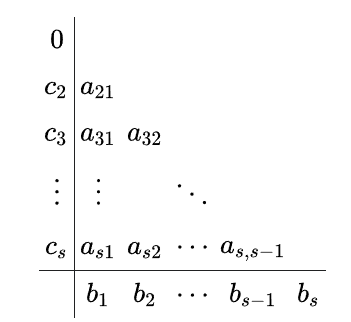
\includegraphics[width=0.3\textwidth]
    {images/butcher_tableau.png}
    \label{fig:my_label}
\end{figure}

The main problem of the methods above is dealing with potential singularities that arise from the superpositioning of two different particles. It is clear from (\ref{gravitational_force}) that the gravitational force diverges in such a case, therefore it is crucial to avoid superpositioning with a precise rationale. These events are extremely rare in real life cases, but can still arise in simulations. One way to tame this is adopting an adaptive numerical method, e.g. Runge-Kutta-Fehlberg, which features an adaptive integration step size. The time step is increasingly shrank as the distance between particles gets smaller, allowing for a better approximation of their positions. 

\section{Algorithmic Approach}
\subsection{Direct-Sum Algorithm}
The straightforward implementation of the n-body problem requires to compute the force between all particles pairwise. This consists in looping over all the bodies at each time step and call the method for gravitational force computation on each object of type \textit{Particle}. In order to do this we need two nested loops. We can avoid performing redundant calculations by updating the force exerted on both particles at once, so that in the inner loop index is initialized as outer index plus one. 
The following pseudo-code is intended for a two dimensional implementation, but can be easily generalized to three dimensions. \cite{PACHECO2022361} \\ \\ \\

\begin{comment}
\begin{figure} [h]
    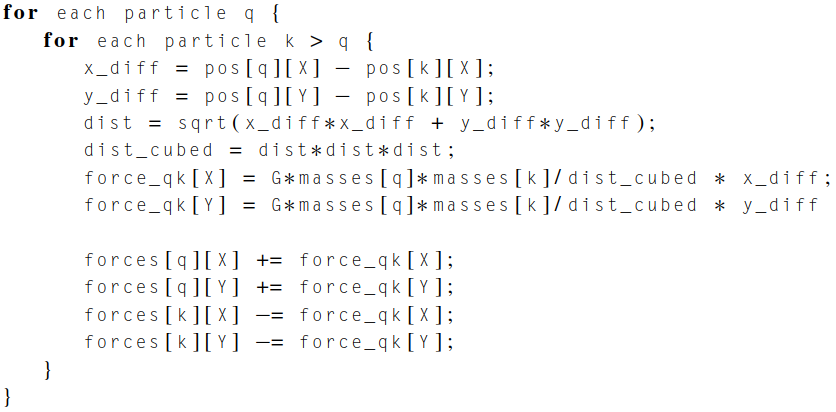
\includegraphics[width=0.8\textwidth]
    {images/nbody_base_algo.png}
    \label{fig:my_label}
\end{figure}
\end{comment}

\begin{boxA}
\begin{verbatim}
    for each particle q
        forces [ q ] = 0;
    for each particle q {
        for each particle k > q {
            x_diff = pos [ q ] [ X ] - pos [ k ] [ X ] ;
            y_diff = pos [ q ] [ Y ] - pos [ k ] [ Y ] ;
            dist = sqrt ( x_diff * x_diff + y_diff * y_diff ) ;
            dist_cubed = dist * dist * dist ;
            force_qk [ X ] = G * masses [ q ] * masses [ k ] / dist_cubed * x_diff ;
            force_qk [ Y ] = G * masses [ q ] * masses [ k ] / dist_cubed * y_diff
            forces [ q ] [ X ] += force_qk [ X ] ;
            forces [ q ] [ Y ] += force_qk [ Y ] ;
            forces [ k ] [ X ] -= force_qk [ X ] ;
            forces [ k ] [ Y ] -= force_qk [ Y ] ;
}
\end{verbatim}
\end{boxA}

\noindent The \textbf{time complexity} of the structure above is $O(n^2)$, since the outer loop runs n times and the inner loop runs n-1, n-2, \dots, 0 times. That is, on average, $\frac{n}{2}$ times, which yields a number of operations of  $\frac{n^2}{2}$. \\

\subsection{Barnes-Hut Algorithm}
In many astronomical scenarios, hierarchical structures exist, such as stars orbiting within galaxies or planets orbiting within a solar system. Hierarchical methods, like the Barnes-Hut algorithm, exploit this structure to reduce the computational complexity of the simulation. \\

The Barnes-Hut simulation, named after Josh Barnes and Piet Hut, divides the three dimensional domain into cubic cells via an \textit{octree}, a particular kind of tree where each node has exactly eight children. It features an algorithm that recursively divides the n bodies into groups and stores them inside the octree. Each node, called octant, corresponds to a precise spacial region. The root of the tree represents the whole 3D domain, while its eight children correspond to the eight octants of the total volume. The whole space is recursively partitioned until each external node, also known as leaf, contains 0 or 1 particles. The denser the body distribution in a certain area, the greater the tree height corresponding to that spacial region. \\

\begin{figure} [h]
    \centering
    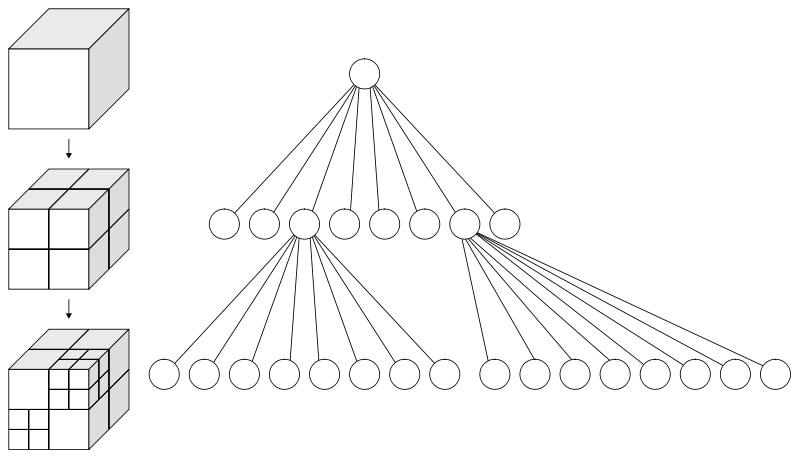
\includegraphics[width=0.5\textwidth]
    {images/octree.png}
    \label{fig:my_label}
    \caption*{Octree, each node has eight children}
\end{figure}

In order to compute the force exerted on a particle, the tree is traversed starting from the root. Whether we should explore it further or not depends on the computation of the so called \textit{multiple acceptance criterion}: \[\theta = \frac{s}{d}\] \\
\noindent where s is the size of the current octant, ergo the spatial region it represents, and d is the distance between its center of mass and the particle that we are considering. At each step of the octree exploration we compute $\theta$;if it's below a given threshold, we consider the whole node as a single particle, with total mass the sum of all the particle masses it contains, and location in its center of mass. This way we drastically reduced the number of force computations for particles that are faraway from each other. The value of $\theta$ determines the accuracy of the simulation, hence the degree of approximation introduced by the algorithm. Note that $\theta = 0$ corresponds to the direct-sum algorithm previously illustrated. \\
This approach yields a \textbf{complexity reduction} from $O(n^2)$ to $O(n \hspace{2pt} lg \hspace{1pt} n)$. \cite{pfalzner1997many}
The pseudo code for the Barnes-Hut recursive insertion algorithm is the following. 

\begin{boxA}
\begin{verbatim}
Function TreeNode::BuildTree
{
    ResetTree

    for all particles
        rootNode->InsertParticle(particle);
    end
}

Function TreeNode::InsertParticle(particle) \\
{
    if particle_number in the node $>$ 1 \\
    {
        octant = GetOctant(particle);

        if child_node(octant) is nullptr
            CreateOctant(octant);

        child_node(octant)->InsertParticle(particle);
    }
    else if particle_number in the node == 1
    {
        octant = GetOctant(storedParticle);
        if child_node(octant) is nullptr 
            CreateOctant(octant);
        child_node->InsertParticle(storedParticle);
        
        octant = GetOctant(particle);
        if child_node(octant) is nullptr 
            CreateOctant(octant);
        child_node->InsertParticle(particle);
    }
    else if particle_number in the node == 0
    {
        storedParticle = particle;
    }
    
    particle_number++;
}
\end{verbatim}
\end{boxA} 

\newpage
The pseudo-code for the force computation relies on the MAC coefficient $\theta$ to calibrate the approximation, which again consists in treating body clusters as single particles.
\begin{boxA}
\begin{verbatim}
Function TreeNode::ComputeForce
{
    if particle_number == 1
        computeAcceleration();
    else 
    {
        r = distance between particle; 
        d = size of the node;

        if(d/r < theta)
        {
            computeAcceleration();
        }
        else 
        {
            for every child octant of the node
            {
             if octant is not nullptr
                force += computeForce();
            }
        }    
    }
}
\end{verbatim}
\end{boxA}

\newpage
\section{Complexity Analysis}
\subsection{Speedup tests}
We performed several simulations to gather data about the speed up achieved with both parallel direct-sum algorithm and parallel Barnes-Hut algorithm. It should be noted that for large number of particles ($>$1000) we didn't run the sequential version, since it would have taken too much time. 
All the tests were run on a machine with 8 cores AMD Ryzen 7 5700U CPU, 24GB of memory and a RTX 3050 Ti Nvidia GPU. The maximum number of available threads is 16.
Moreover, all the tests excluded the operation of writing the results to a file through the \textbf{exporter} class, since this is intrinsically sequential. We made sure that were as few processes in the background as possible, in order to avoid polluting the results. \\
\subsubsection{Sequential vs Parallel Direct-Sum} First we performed some small tests to assess the speedup between the sequential and OpenMP parallel versions of the direct-sum algorithm. For the latter we expect some performance loss due to the presence of atomic instructions that ensure the consistency of the force computation. In addition to that, all threads that have been spawned need to synchronize at the end of each parallel construct, since they all have an implicit barrier at their exiting point. \\
For small tests, we ran the simulation multiple times to ensure that the results were consistent, so as to extract an average of the execution time and reduce the performance oscillations due to processes running in the background. The number of time steps of each simulation gets lower as the number of particles increases. The amount of time steps for small sets of bodies must be sufficiently high, otherwise the simulation is too short and results may be inaccurate. The time unit is \textit{milliseconds}. \\

\begin{boxA}
    \begin{verbatim}
# 128 particles / 8000 time steps
Average parallel execution time with 2 threads: 1065.8 
Average parallel execution time with 4 threads: 728.6
Average parallel execution time with 6 threads: 580.4
Average parallel execution time with 8 threads: 523
Average parallel execution time with 12 threads: 457.8
Average parallel execution time with 16 threads: 496
Average serial execution time: 910.8
Average speed up with 2 threads: 0.85
Average speed up with 4 threads: 1.25
Average speed up with 6 threads: 1.57
Average speed up with 8 threads: 1.741
Average speed up with 12 threads: 1.99
Average speed up with 16 threads: 1.83
\end{verbatim}
\end{boxA}

\begin{boxA}
    \begin{verbatim}
# 512 / 2000 time steps
Average parallel execution time with 2 threads: 3859.8
Average parallel execution time with 4 threads: 2234.8
Average parallel execution time with 6 threads: 1666
Average parallel execution time with 8 threads: 1338.4
Average parallel execution time with 12 threads: 1007.6
Average parallel execution time with 16 threads: 937.8
Average serial execution time: 3617
Average speed up with 2 threads: 0.94
Average speed up with 4 threads: 1.61
Average speed up with 6 threads: 2.17
Average speed up with 8 threads: 2.70
Average speed up with 12 threads: 3.58
Average speed up with 16 threads: 3.85
\end{verbatim}
\end{boxA}

\begin{boxA}
    \begin{verbatim}
# 4096 particles / 100 time steps
Average parallel execution time with 2 threads: 11886
Average parallel execution time with 4 threads: 6333.6
Average parallel execution time with 6 threads: 4577.4
Average parallel execution time with 8 threads: 3544.6
Average parallel execution time with 12 threads: 2568.8
Average parallel execution time with 16 threads: 2176
Average serial execution time: 11620.2
Average speed up with 2 threads: 0.97
Average speed up with 4 threads: 1.83
Average speed up with 6 threads: 2.53
Average speed up with 8 threads: 3.27
Average speed up with 12 threads: 4.52
Average speed up with 16 threads: 5.34
\end{verbatim}
\end{boxA}

\begin{boxA}
    \begin{verbatim}
# 16,384 particles / 1 time step
Average parallel execution time with 2 threads: 1938.8
Average parallel execution time with 4 threads: 997.2
Average parallel execution time with 6 threads: 683
Average parallel execution time with 8 threads: 531.6
Average parallel execution time with 12 threads: 384.6
Average parallel execution time with 16 threads: 337.6
Average serial execution time: 1873.6
Average speed up with 2 threads: 0.96
Average speed up with 4 threads: 1.87
Average speed up with 6 threads: 2.74
Average speed up with 8 threads: 3.52
Average speed up with 12 threads: 4.87
Average speed up with 16 threads: 5.54
\end{verbatim}
\end{boxA}

Let us sum up and visualize the results on a plot to better understand the speedup trend with respect to the number of OpenMP threads. On the x axis we depict the number of working threads, while on the y axis we represent the corresponding speedup.All the plots that follow have been produced with a simple Python script. 

\begin{figure} [h]
    \centering
    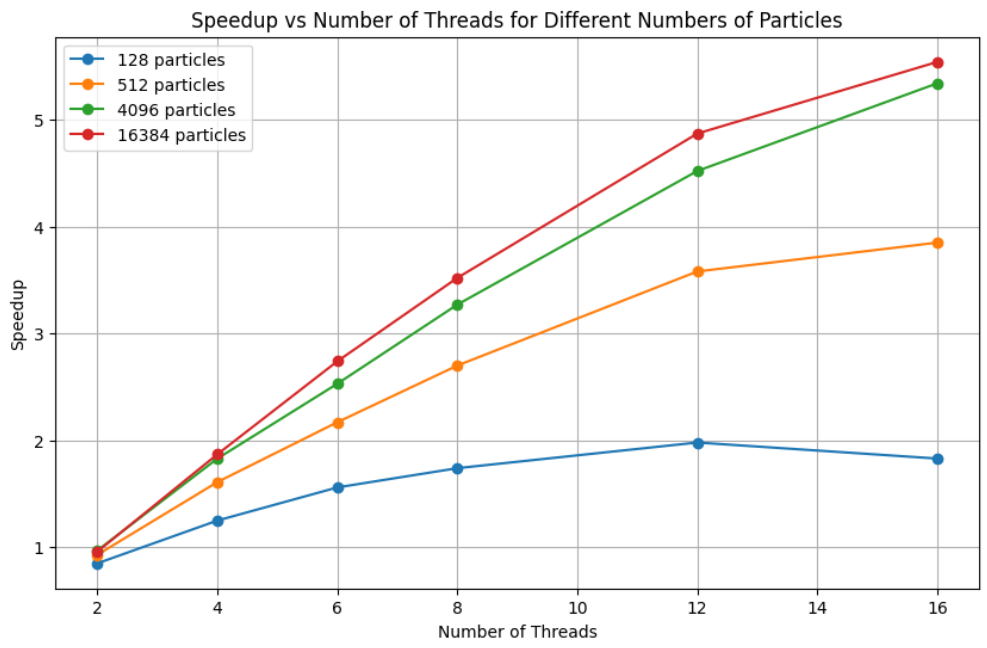
\includegraphics[width=1\textwidth]
    {images/serial_parallel_speedup.png}
    \label{fig:execution_time}
    % \caption*{Octree, each node has eight children}
\end{figure}

For a small number of bodies, we expect and actually obtain some performance degradation with a number of threads too high. This is due to the fact that each thread is assigned a workload too small with respect to the its creation and synchronization costs. For larger systems, we didn't manage to reach a degradation or even a plateau, since we have just 16 hardware threads at our disposal on the machine that runs the simulations. 

\subsubsection{Direct-sum vs Barnes-Hut}
Now we shall take into consideration the comparison between the parallel version of both direct-sum and Barnes-Hut algorithm. We expect the performance of the latter to get better for higher values of the multipole acceptance criterion, while the accuracy gets lower.In addition to that, Barnes-Hut performs better with an increasing number of particles. This is due to the fact that handling the octree has an intrinsic cost, which is well amortized when the body number is at least in the order of $10^4$.

Now a bigger test over a limited number of time steps, which are not really relevant for the scope of our analysis.
\begin{boxA}
\begin{verbatim}
# 16384 particles / 3600 timesteps 
Time taken by DS parallel execution: 1350 seconds
Theta = 0.5 - Time taken by BH execution: 437 seconds
Speedup: 3.09
Theta = 0.7 - Time taken by BH execution: 286 seconds
Speedup: 4.70
Theta = 1 - Time taken by BH execution: 180 seconds
Speedup: 7.46
\end{verbatim}
\end{boxA}

We'd like to scale up the numbers even more, but we need to sacrifice the number of step simulations to be able to do that. Let us compare the speed up with the same number of particles, over just one time step. We obtain the following results, which are frankly quite comforting: \\
\begin{boxA}
\begin{verbatim}
# 16384 particles / 1 timesteps

Average parallel execution time: 150 milliseconds
Average BH execution time for theta = 0.5: 49.4 milliseconds
Average BH execution time for theta = 0.7: 29.8 milliseconds
Average BH execution time for theta = 1.0: 20.6 milliseconds
Average speed up with theta = 0.5: 3.03
Average speed up with theta = 0.7: 5.04
Average speed up with theta = 1.0: 7.29
\end{verbatim}
\end{boxA}
\noindent Note that the net execution time is not proportional since in the first case the computer wasn't connected to the power supply and was running the simulation with more processes in the background. This caused the former simulation to be slower at computing a single time step. All the following tests were performed with as little interference from other programs as possible. Nevertheless, we can conclude that the number of time steps is approximately irrelevant for the performance evaluation thanks to the speedup values, which are analogous in both cases.This allows us to simulate quite big systems even on a single machine. Let us simulate a number of bodies from $2^{15}$ to $2^{19}$ over just one step. 

\begin{boxA}
    \begin{verbatim}
# 32768 particles / 1 timesteps
Average parallel execution time: 1324.4 milliseconds
Average BH execution time for theta = 0.5: 367.4 milliseconds
Average BH execution time for theta = 0.7: 209.4 milliseconds
Average BH execution time for theta = 1.0: 142.4 milliseconds
Average speed up with theta = 0.5: 3.68
Average speed up with theta = 0.7: 6.33
Average speed up with theta = 1.0: 9.31
\end{verbatim}
\end{boxA}

\begin{boxA}
    \begin{verbatim}
# 65536 particles / 1 timesteps
Average parallel execution time: 10725.6 milliseconds
Average BH execution time for theta = 0.5: 2058.2 milliseconds
Average BH execution time for theta = 0.7: 1116 milliseconds
Average BH execution time for theta = 1.0: 733.8 milliseconds
Average speed up with theta = 0.5: 5.32
Average speed up with theta = 0.7: 9.71
Average speed up with theta = 1.0: 14.61
\end{verbatim}
\end{boxA}

\begin{boxA}
    \begin{verbatim}
# 131072 particles / 1 timesteps
Average parallel execution time: 30625.6 milliseconds
Average BH execution time for theta = 0.5: 2496.6 milliseconds
Average BH execution time for theta = 0.7: 1345.4 milliseconds
Average BH execution time for theta = 1.0: 860.6 milliseconds
Average speed up with theta = 0.5: 12
Average speed up with theta = 0.7: 22
Average speed up with theta = 1.0: 35
\end{verbatim}
\end{boxA}

\begin{boxA}
    \begin{verbatim}
# 262144 particles / 1 timesteps
Average parallel execution time: 144.48 seconds
Average BH execution time for theta = 0.5: 5.33 seconds
Average BH execution time for theta = 0.7: 2.69 seconds
Average BH execution time for theta = 1.0: 1.60 seconds
Average speed up with theta = 0.5: 27
Average speed up with theta = 0.7: 53
Average speed up with theta = 1.0: 91
\end{verbatim}
\end{boxA}

\begin{boxA}
    \begin{verbatim}
# 524288 particles / 1 timesteps
Average parallel execution time: 851.8 seconds
Average BH execution time for theta = 0.5: 12.4 seconds
Average BH execution time for theta = 0.7: 6.4 seconds
Average BH execution time for theta = 1.0: 3.7 seconds
Average speed up with theta = 0.5: 68
Average speed up with theta = 0.7: 133
Average speed up with theta = 1.0: 230
    \end{verbatim}
\end{boxA}

\noindent It can be clearly observed that the larger the number of bodies, the better the BH algorithm performs. This is to be expected since the complexity is \textit{quadratic} for DS and \textit{superlinear} for BH. The results can be summarized in the following plots. First we represent the execution time of the four different versions, namely direct-sum (DS), Barnes-Hut with $\theta = 0.5$ (BH05), $\theta = 0.7$ (BH07) and $\theta = 1.0$ (BH1). The increasing numbers of bodies are the same as above. \\

\begin{figure} [h]
    \centering
    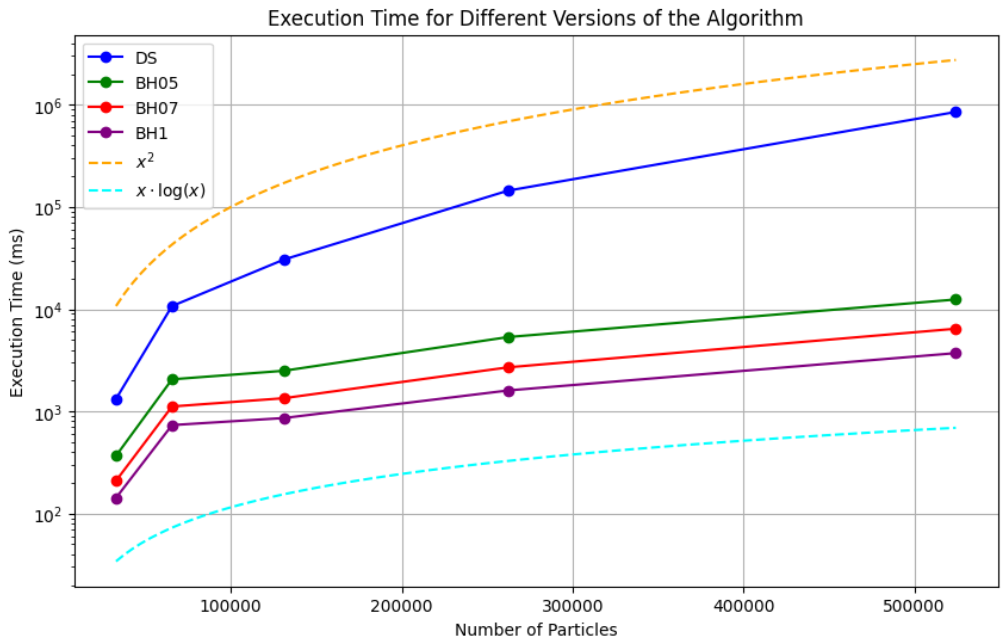
\includegraphics[width=1\textwidth]
    {images/BH_DS_comparison.png}
    \label{fig:execution_time}
    % \caption*{Octree, each node has eight children}
\end{figure}

\noindent It can be easily noted that for large enough datasets, Barnes-Hut reduces the computation time by different orders of magnitude. This constitutes a huge improvement with respect to the initial parallel implementation. The plot confirms that the actual complexity is very close to the theoretical one, which has been traced on the graph.
\noindent Then we shall produce a plot of the speedup of Barnes-Hut with respect to the direct-sum version, for different values of $\theta$ and increasing numbers of bodies.

\begin{figure} [h]
    \centering
    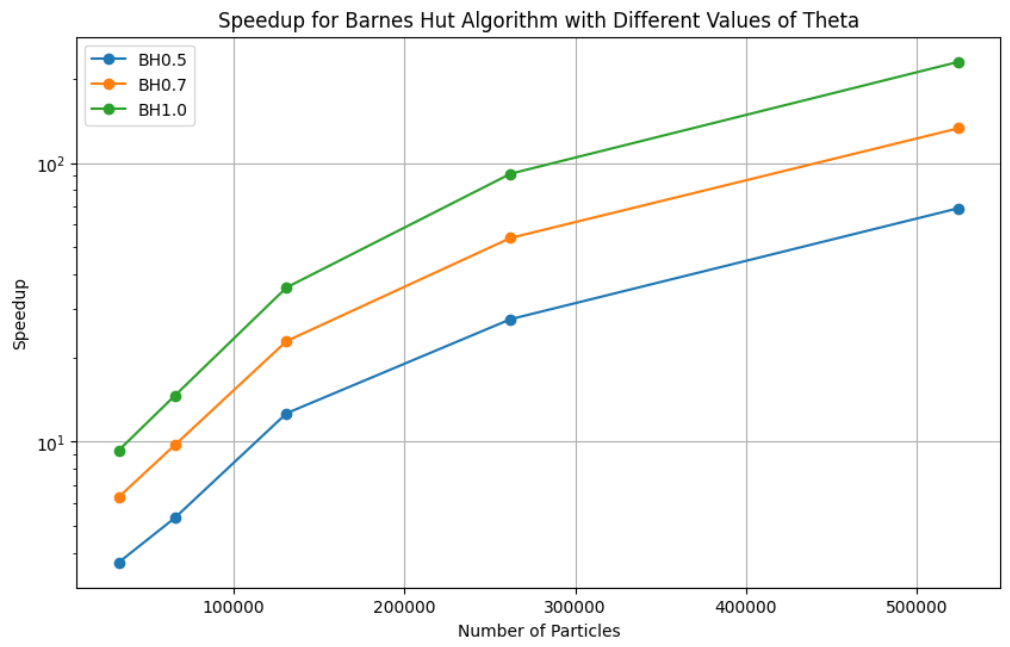
\includegraphics[width=1\textwidth]
    {images/BH_speedup.png}
    \label{fig:BH_speedup}
    % \caption*{Octree, each node has eight children}
\end{figure}

\newpage
\section{Results Visualization}
The first approach consisted in using python libraries, namely pyplot and matplotlib.animation. This is a very simplified approach due to their wide use and accessible features, though the result wasn't the most satisfactory from a graphical perspective. First of all the file must be parsed in order to extract the positions of the particles over time. This is done by the \textbf{parser.py} file. We created a .part format, which stores information in the following way: \\
\begin{verbatim}
--- timeInstant
PART0 pos.x pos.y pos.z
PART1 pos.x pos.y pos.z
\end{verbatim}
An example would be:
\begin{verbatim}
---0
PART0 -0.629132 -0.0166424 -0.58994
PART1 -1.70392 -0.281137 4.8288
\end{verbatim}

\noindent The output of the parser becomes the input of \textbf{viewer.py}, which actually renders the graphic simulation. 
A screenshot of a simulation looks like this: \\
% insert a decent screenshot
        
Since we weren't satisfacted with the result, we opted for another solution. We chose an external library named \textit{OpenFrameworks}, cross platform toolkit for creative coding in C++. It is actually a wrapper built on top of OpenGL, a well-known platform for rendering 2D and 3D vector graphics. We added OpenFrameworks to our repository as a submodule, so that its linking with our project is immediate. The process of installing and compiling the library is quite tedious, but it's definitely worth it. The installation and compilation procedure is reported in the repository. We decided to use an addon named \textit{Bloom} to add some style to the bodies. Its implementation can be found at \url{https://github.com/P-A-N/ofxBloom}. The structure of our OpenFrameworks project is as follows:
\begin{verbatim}
ofApp.hpp  --> declaration of OF functions and members useful for the simulation
ofApp.cpp  --> definitions of such functions, implementation of the graphic rendering
Parser.hpp --> C++ parser to process the input .part file
main.cpp   --> calls the parser and triggers the visualization process 
\end{verbatim}


The visualization process in OpenFrameworks is quite straightforward.
First the \textit{setup()} method initializes the OpenGL platform and creates a graphic window of the right dimensions.
The \textit{update()} method is called at every step of the simulation and allows it to evolve over time. It eventually resets it once it reaches the end. The \textit{draw()} method is designated with the actual rendering of the bodies. It initializes the camera and extracts the positions of the particles at the current time step. Then it draws a spherical object for each body, colors it and scales it to the window dimensions. \\

\newpage When it comes to producing a graphic visualization of a simulation, the numbers need to be contained. This is due to the cost of computing the evolution of the system over a large time span and the size of the output file. The following screenshot has been taken at time step 33,228 over a total of 86,400 during a simulation of 1024 particles. They were generated randomly and arranged in four cubic shapes. The clusters begin to spin and rotate clockwise until and progressively collide and merge with each other, producing nice visual effects. The full video of the simulation can be found \href{https://github.com/AMSC22-23/N-Body-simulator/tree/main/examples/example_OF}{here}. 

\begin{figure} [h]
    \centering
    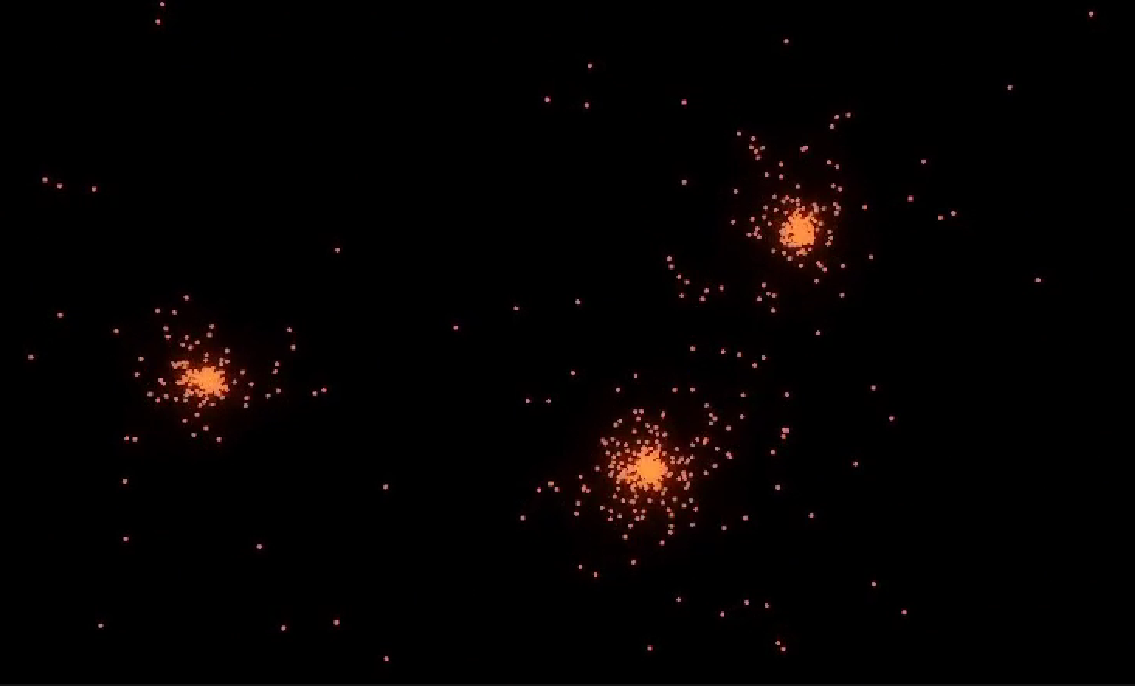
\includegraphics[width=1\textwidth]
    {images/definitive_simulation.png}
    \label{fig:my_label}
\end{figure}

It can be noted that several particles are thrown outside the simulation due to gravitational slingshot phenomenon and instability in close quarters interactions. This is normal since the numerical integration methods that we implemented do not feature an adaptive time step, which would diminish divergence when the distance between bodies tends to zero. Nevertheless, the result is quite satisfactory.

\newpage
\printbibliography

\end{document}

